\section{Sepia}


\subsection{Descripción}

El filtro sepia consiste en cambiar los colores de cada pixel de la siguiente manera:

$$ O^r_{i,j} = 0,5 \cdot suma_{i,j} $$
$$ O^g_{i,j} = 0,3 \cdot suma_{i,j} $$
$$ O^b_{i,j} = 0,2 \cdot suma_{i,j} $$
$$ O^a_{i,j} = I^a_{i,j} $$

donde $suma_{i,j} = I^r_{i,j} + I^g_{i,j} + I^b_{i,j}$

Como puede verse, este filtro no recibe ningún parámetro y trabaja directamente con los datos mismos de la imagen.

\subsection{Implementaciones}

Antes de entrar en detalle a cada una de las implementaciones hechas, es importante notar que

$$suma_{i,j} = I^r_{i,j} + I^g_{i,j} + I^b_{i,j} \leq 255 + 255 + 255 = 3 \cdot 255$$

Lo cual excede el rango de representación de las componentes de un pixel. Esto puede resultar en un problema o no dependiendo de cada caso, ya que es necesario calcular $suma_{i,j}$ para resultados intermedios. Como el resultado final de aplicar el filtro en cada componente es multiplicar $suma_{i,j}$ por un número menor o igual a 1, se consideró aplicar la ley distributiva para poder salvar este problema, ya que, por ejemplo, en el caso de la componente azul

$$ O^b_{i,j} = 0,2 \cdot suma_{i,j} = 0,2 \cdot (I^r_{i,j} + I^g_{i,j} + I^b_{i,j}) = 0,2 \cdot I^r_{i,j} +  0,2 \cdot I^g_{i,j} + 0,2 \cdot I^b_{i,j} \leq 0,2 \cdot 255 + 0,2 \cdot 255 + 0,2 \cdot 255 = 0,6 \cdot 255 \leq 255$$


y en el caso de la componente verde

$$ O^b_{i,j} = 0,3 \cdot suma_{i,j} = 0,3 \cdot (I^r_{i,j} + I^g_{i,j} + I^b_{i,j}) = 0,3 \cdot I^r_{i,j} +  0,3 \cdot I^g_{i,j} + 0,3 \cdot I^b_{i,j} \leq 0,3 \cdot 255 + 0,3 \cdot 255 + 0,3 \cdot 255 = 0,9 \cdot 255 \leq 255$$

Cabe resaltar que realizando las operaciones de este modo, nunca se llega a un resultado intermedio el cual exceda el límite de representación de las componentes.

Sin embargo, esta alternativa fue descartada ya que implica hacer el triple de multiplicaciones en punto flotante, lo cual reduce drásticamente la performance.

Además, se debe notar que en el caso de la componente roja ocurre lo siguiente:

	$$ O^b_{i,j} = 0,5 \cdot suma_{i,j} \leq 0,5 \cdot 3 \cdot 255 = 1,5 \cdot 255$$

Lo cual resulta un problema a la hora de almacenar el resultado final ya que el mismo podría exceder el rango de representación de la componente roja. En cada una de las implementaciones se detalla cómo fue resuelta esta cuestión.

\subsubsection{C}

A grandes rasgos, la implementación en C es intuitiva, ya que recorre cada uno de los píxeles uno por uno, por cada iteración crea una variable auxiliar llamada $suma$ (la cual, como puede esperarse, contiene el valor de $suma_{i,j}$) y asigna a cada componente el valor de dicha suma multiplicada por su respectivo factor.
Debido a las dos problemáticas que se plantearon anteriormente, se hicieron algunos ajustes con respecto a la implementación. La variable auxiliar $suma$ es una variable del tipo $unsigned short (16 bits)$  para no perder precisión en las operaciones. Por la misma razón, se creó también una nueva variable auxiliar $suma_r$, la cual contiene el valor de $0,5 \cdot suma_{i,j} = I^r_{i,j}$.
Para volver a $char (8 bits)$ se resuelve distinto en cada caso.
\begin{itemize}
	\item En el caso de $suma$ con respecto a las componentes azul y verde, solamente se les asigna a cada una el valor de $suma$ multiplicado por su respectivo factor ya que, como se demostró anteriormente, $O^b_{i,j}$ y $O^g_{i,j}$ son siempre menores a 255 y por lo tanto no hay que tener ningún recaudo extra. Luego de ejecutar la multiplicación, el lenguaje C simplemente convierte el dato a $char$ y lo asigna.
	\item En el caso de $suma_r$, se pregunta primero si el resultado final dio mayor o igual a 255. Si eso es cierto, lo satura a 255. Caso contrario, lo deja como está. En esencia se está ejecutando un $min(I^r_{i,j},255)$.
\end{itemize}

La cantidad de operaciones de punto flotante por pixel en esta implementación es de $\frac{3op}{px}$.

\subsubsection{Asm - SSE}

Cada componente ocupa 1 byte y cada pixel tiene 4 componentes, por lo cual un pixel ocupa 4 bytes. Como los registros \xmm{} son de 16B, es posible procesar 4 píxeles en un solo registro simultáneamente.
Al inicio del loop, se copian 4 píxeles de la imagen fuente a \xmm{0} para empezar a procesar. Para simplificar la notación, se llamará $K_{i}$ a la componente K del pixel $i \in {0,1,2,3}$

\xmm{0} \xmmByte{$A_{3}$}{$R_{3}$}{$G_{3}$}{$B_{3}$}{$A_{2}$}{$R_{2}$}{$G_{2}$}{$B_{2}$}{$A_{1}$}{$R_{1}$}{$G_{1}$}{$B_{1}$}{$A_{0}$}{$R_{0}$}{$G_{0}$}{$B_{0}$}

Luego, se copia a \xmm{1} y \xmm{3} el contenido de \xmm{0} y se borran los alpha de los mismos

\xmm{1} \xmmByte{$0$}{$R_{3}$}{$G_{3}$}{$B_{3}$}{$0$}{$R_{2}$}{$G_{2}$}{$B_{2}$}{$0$}{$R_{1}$}{$G_{1}$}{$B_{1}$}{$0$}{$R_{0}$}{$G_{0}$}{$B_{0}$}

\xmm{3} \xmmByte{$0$}{$R_{3}$}{$G_{3}$}{$B_{3}$}{$0$}{$R_{2}$}{$G_{2}$}{$B_{2}$}{$0$}{$R_{1}$}{$G_{1}$}{$B_{1}$}{$0$}{$R_{0}$}{$G_{0}$}{$B_{0}$}

Se desempaquetan \xmm{1} y \xmm{3} de tal manera que \xmm{1} tenga la parte baja y \xmm{3} la parte alta. Ambos terminarían convirtiéndose en registros de words empaquetados. Esto se hace con el fin de poder luego ejecutar una suma horizontal de a word sin el riesgo de que el resultado quede fuera del rango de representación.

\xmm{1} \xmmWord{$0$}{$R_{1}$}{$G_{1}$}{$B_{1}$}{$0$}{$R_{0}$}{$G_{0}$}{$B_{0}$}

\xmm{3} \xmmWord{$0$}{$R_{3}$}{$G_{3}$}{$B_{3}$}{$0$}{$R_{2}$}{$G_{2}$}{$B_{2}$}

Se ejecutan las sumas horizontales necesarias para que \xmm{1} tenga el resultado

\xmm{1} \xmmWord{$0$}{$0$}{$0$}{$0$}{$S_{3}$}{$S_{2}$}{$S_{1}$}{$S_{0}$}

donde $S_{i} = R_{i} + G_{i} + B_{i}$

Se convierte \xmm{1} a float para poder realizar la multiplicación por los factores correspondientes, y luego se ejecutan varios shuffle de tal manera que haya un registro completo por cada pixel

\xmm{1} \xmmFloat{$S_{0}$}{$S_{0}$}{$S_{0}$}{$S_{0}$}

\xmm{2} \xmmFloat{$S_{1}$}{$S_{1}$}{$S_{1}$}{$S_{1}$}

\xmm{3} \xmmFloat{$S_{2}$}{$S_{2}$}{$S_{2}$}{$S_{2}$}

\xmm{4} \xmmFloat{$S_{3}$}{$S_{3}$}{$S_{3}$}{$S_{3}$}

Se multiplica a los cuatro registros por el siguiente vector de factores que se encuentra alojado en \xmm{15}

\xmm{15} \xmmFloat{$0$}{$0,5$}{$0,3$}{$0,2$}

Lo cual da como resultado

\xmm{1} \xmmFloat{$0$}{$0,5 \cdot S_{0}$}{$0,3 \cdot S_{0}$}{$0,2 \cdot S_{0}$}

\xmm{2} \xmmFloat{$0$}{$0,5 \cdot S_{1}$}{$0,3 \cdot S_{1}$}{$0,2 \cdot S_{1}$}

\xmm{3} \xmmFloat{$0$}{$0,5 \cdot S_{2}$}{$0,3 \cdot S_{2}$}{$0,2 \cdot S_{2}$}

\xmm{4} \xmmFloat{$0$}{$0,5 \cdot S_{3}$}{$0,3 \cdot S_{3}$}{$0,2 \cdot S_{3}$}

Es decir

\xmm{1} \xmmFloat{$0$}{$O^r_{0}$}{$O^g_{0}$}{$O^b_{0}$}

\xmm{2} \xmmFloat{$0$}{$O^r_{1}$}{$O^g_{1}$}{$O^b_{1}$}

\xmm{3} \xmmFloat{$0$}{$O^r_{2}$}{$O^g_{2}$}{$O^b_{2}$}

\xmm{4} \xmmFloat{$0$}{$O^r_{3}$}{$O^g_{3}$}{$O^b_{3}$}

Se reconvierte cada registro a int y se empaquetan de manera saturada los datos en \xmm{1}. La saturación es la solución al overflow de la componente roja, ya que la instrucción misma la transforma en 255 en caso de ser mayor.

\xmm{1} \xmmByte{$0$}{$O^r_{3}$}{$O^g_{3}$}{$O^b_{3}$}{$0$}{$O^r_{2}$}{$O^g_{2}$}{$O^b_{2}$}{$0$}{$O^r_{1}$}{$O^g_{1}$}{$O^b_{1}$}{$0$}{$O^r_{0}$}{$O^g_{0}$}{$O^b_{0}$}

Por el lado de \xmm{0}, se eliminan los datos de los colores y se deja solo el alpha para poder luego "fusionar" los datos con \xmm{1}

\xmm{0} \xmmByte{$A_{3}$}{$0$}{$0$}{$0$}{$A_{2}$}{$0$}{$0$}{$0$}{$A_{1}$}{$0$}{$0$}{$0$}{$A_{0}$}{$0$}{$0$}{$0$}

Por último, se unen los datos de \xmm{0} y \xmm{1} y se almacena en la imagen destino.

\xmm{0} \xmmByte{$O^a_{3}$}{$O^r_{3}$}{$O^g_{3}$}{$O^b_{3}$}{$O^a_{2}$}{$O^r_{2}$}{$O^g_{2}$}{$O^b_{2}$}{$O^a_{1}$}{$O^r_{1}$}{$O^g_{1}$}{$O^b_{1}$}{$O^a_{0}$}{$O^r_{0}$}{$O^g_{0}$}{$O^b_{0}$}

La cantidad de operaciones de punto flotante por pixel en esta implementación es de $\frac{4op}{4px} = \frac{1op}{px}$, La cual es menor comparado a la cantidad de operaciones por pixel de la implementación en C (la cual es $\frac{3op}{px}$).

\vspace{2mm}

Con la finalidad de aumentar el rendimiento de esta implementación, se decidió utilizar más registros para procesar más cantidad de memoria en un mismo loop, de modo tal que la ejecución fuera de orden fuera más efectiva y se realice la menor cantidad de saltos condicionales posible.

Como se pudo ver en el desarrollo del algoritmo, solo cinco registros fueron utilizados para realizar todo el proceso (\xmm{0}..\xmm{4}), esto nos permite procesar de a 12 píxeles por ciclo, utilizando 15 de los 16 registros xmm, dejando espacio libre para el registro extra que contiene los factores por los que hay que multiplicar.

También es necesario utilizar un registro lleno de ceros para desempaquetar los datos, lo cual haría necesario contar con 17 registros o acceder a memoria, pero como ese registro de ceros solo es necesario durante una sola parte del algoritmo (en la cual aún no están en uso todos los registros) se puede utilizar algún registro que aún no se haya procesado.

La problemática que surge a partir de procesar de a 12 píxeles, es que no se sabe si se puede estar procesando píxeles de más, ya que solo se tiene como hipótesis que el ancho de la imagen multiplicado por su altura es un número que es múltiplo de 8, y por ende no siempre tendremos una imagen cuyo tamaño total sea múltiplo de 12. Para solucionar esto, se procesa de a 12 píxeles todas las veces que se pueda, y cuando ya no se pueda más, se procesa de a 4 como originalmente se hacía, hasta terminar de procesar toda la imagen. Notar que no puede llegar a ocurrir que el algoritmo haya tenido que procesar de a 4 píxeles más de 2 veces.

\subsubsection{Asm - AVX2}

En AVX2 podemos utilizar los registros extendidos \ymm{} de 256 bits, por lo cual podemos procesar el doble de píxeles que en la implementación SSE. También contamos con instrucciones no destructivas que nos ahorran un par de pasos a la hora de implementar. Por ejemplo, podemos pasar de

\begin{lstlisting}
MOVDQA XMM1, XMM0
PSLLD XMM1, 8
PSRLD XMM1, 8
\end{lstlisting}

a

\begin{lstlisting}
VPSLLD XMM1, XMM0, 8
VPSRLD XMM1, XMM1, 8
\end{lstlisting}


La conversión del algoritmo es directa con respecto a SSE. La estrategia es la misma, con la salvedad de que hay que tener cuidado con algunas instrucciones que no funcionan exactamente igual a su instrucción análoga de SSE.

Por ejemplo, a la hora de convertir los registros a word ejecutando VPUNPCKLBW y VPUNPCKHBW, estos quedarían de la siguiente manera

\begin{lstlisting}
VPUNPCKLBW XMM3, XMM1, XMM7
VPUNPCKHBW XMM1, XMM1, XMM7
\end{lstlisting}

\ymm{1} \ymmWord{$0$}{$R_{5}$}{$G_{5}$}{$B_{5}$}{$0$}{$R_{4}$}{$G_{4}$}{$B_{4}$}{$0$}{$R_{1}$}{$G_{1}$}{$B_{1}$}{$0$}{$R_{0}$}{$G_{0}$}{$B_{0}$}

\ymm{3} \ymmWord{$0$}{$R_{7}$}{$G_{7}$}{$B_{7}$}{$0$}{$R_{6}$}{$G_{6}$}{$B_{6}$}{$0$}{$R_{3}$}{$G_{3}$}{$B_{3}$}{$0$}{$R_{2}$}{$G_{2}$}{$B_{2}$}

Por lo general, en las instrucciones de AVX2 se mantiene la misma estructura que se vio en el reciente ejemplo: Primero se procesa la parte baja de los dos registros fuente, y luego se procesa la parte alta de cada uno, en vez de procesar cada uno por completo a la vez.

Esta implementación ejecuta la misma cantidad de operaciones en punto flotante que SSE, pero procesa el doble de píxeles. Por lo tanto, por cada loop obtenemos un rendimiento de $\frac{4op}{8px} = \frac{1op}{2px}$.


\subsection{Experimentos}

\subsubsection{Comparación entre implementaciones}

 Luego de realizar varias corridas de cada una de las implementaciones, se llegaron a los siguientes resultados en cuanto al tiempo total de ejecución:

\begin{figure}[h]
    \centering
    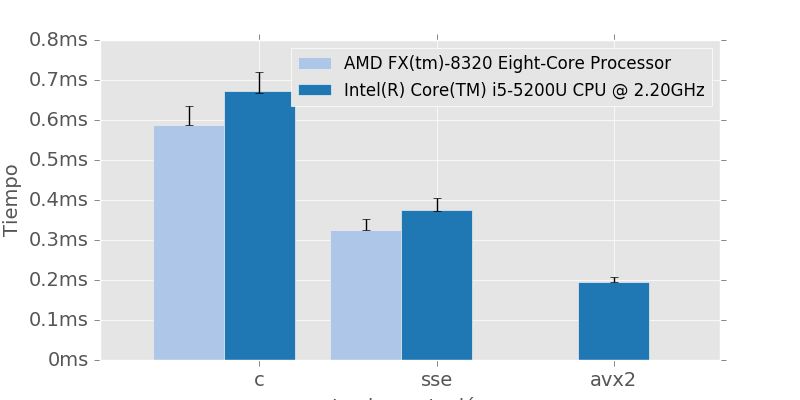
\includegraphics[width=0.9\textwidth]{sepia-time}
    \caption{Tiempo de ejecución del filtro sepia sobre lena.bmp 512x512}
    \label{fig:sepia-time}
\end{figure}

Se puede inferir entonces que las suposiciones anteriores en cuanto a mejoras de performance resultaron ser verdaderas. La implementación en SSE corre más rápido que la misma en C y la implementación en AVX2 corre aún más rápido que SSE.

En el siguiente gráfico se explicita con más detalle qué tanto más rápidas son las dos implementaciones en ASM con respecto a C compilado con la optimización O3:

\begin{figure}[h]
    \centering
    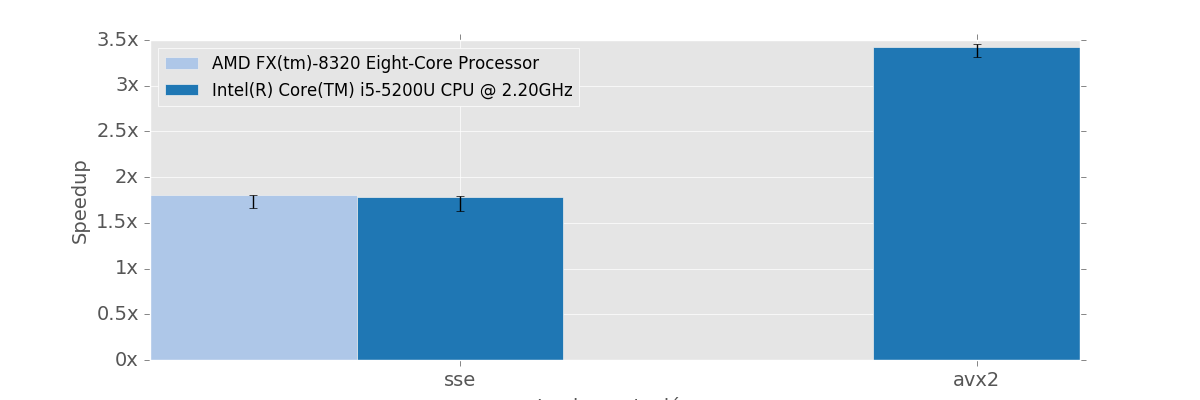
\includegraphics[width=0.9\textwidth]{sepia-time-speedup}
    \caption{Tiempo de ejecución relativo de implementaciones ASM de sepia contra la implementación C compilada con -O3}
    \label{fig:sepia-time-speedup}
\end{figure}

Se puede ver que SSE presenta un speedup de poco menos de 2 y AVX2 presenta un speedup de casi 3.5, evidenciando aún más fuertemente la mejora que se obtiene a medida que se va aumentando el paralelismo del procesamiento de píxeles.

Es importante aclarar que para realizar este experimento, se compiló la implementación en C con la opción de optimización automática O3.

\cuidado \\
Estaria bueno aca que mencionen la cantidad de operaciones por pixel que calcularon antes para cada implementacion. Por ej. C vs SSE hace el triple de operaciones, por lo que sería esperable que funcione alrededor de 3X veces mas lento
\cuidado

\subsubsection{Comparación entre optimizaciones de C}

Las diferencias de performance entre la implementación C sin optimizar (O0) y las distintas optimizaciones se puede apreciar en el siguiente gráfico:

\begin{figure}[h]
    \centering
    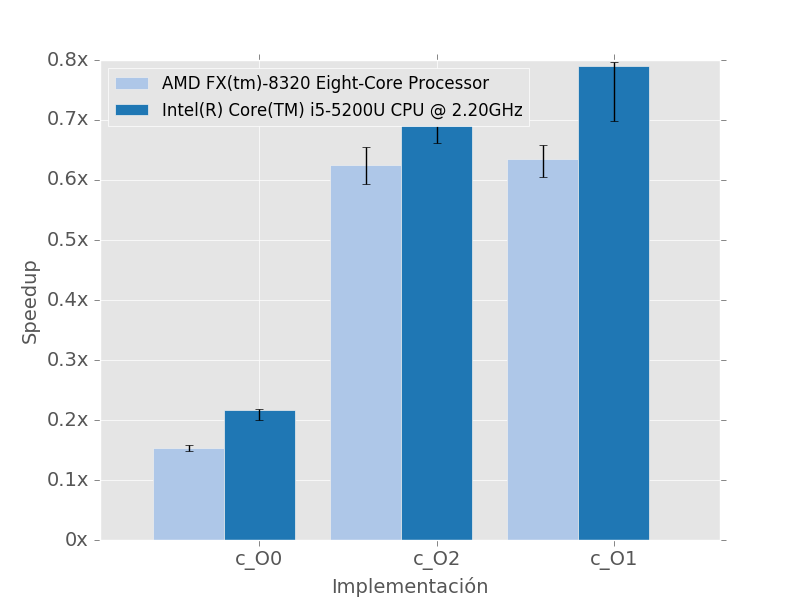
\includegraphics[width=0.9\textwidth]{sepia-c-time-speedup}
    \caption{Tiempo de ejecución relativo de diferentes optimizaciones de la implementación en C respecto a lo optimización O3}
    \label{fig:sepia-c-time}
\end{figure}

Como puede verse, la versión sin optimizar es muchas veces más lenta que la versión completamente optimizada. Es decir que la diferencia entre la implementación en C sin optimizar y las implementaciones en SSE y AVX2 es aún más grande en cuanto a performance.

\subsubsection{Caché misses en función del tamaño de imagen}

Como siguiente cuestión, nos planteamos la pregunta sobre qué tanto porcentaje de Cache Misses se presentan al correr los códigos. Para encontrar una respuesta, decidimos hacer un experimento en el cual surgieron los siguientes resultados para la implementación en SSE:

\begin{figure}[h]
    \centering
    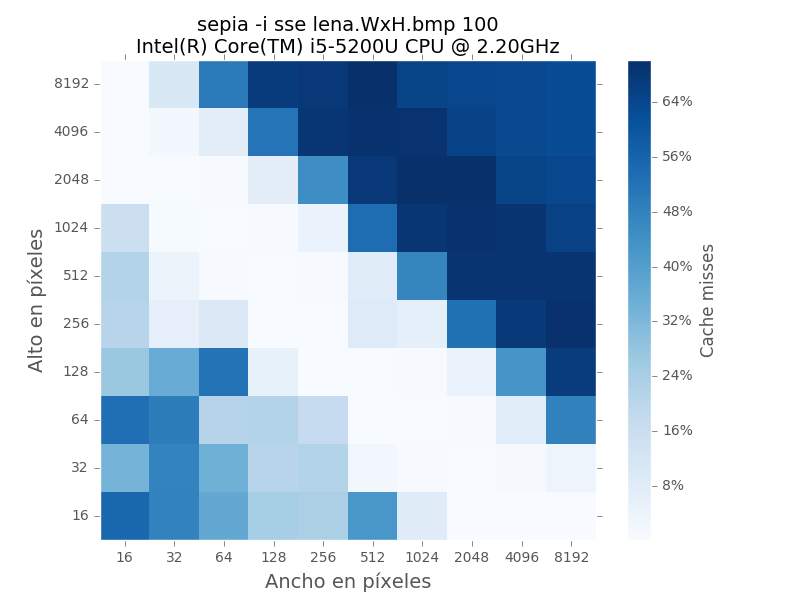
\includegraphics[width=0.65\textwidth]{sepia-cache-map-sse-angua}
    \caption{Porcentaje de caché misses en función del tamaño de imagen al correr el filtro sepia en un procesador con 3MB de caché}
    \label{fig:sepia-cache-map-sse-angua}
\end{figure}

Los casos que se encuentran alrededor de 128x128 tienen un miss rate ligeramente menor debido a que varios píxeles ya se encontraban en cache a la hora de volver a testear la misma imagen pero con distinto tamaño. Luego, al aumentar el ancho o el alto de la imagen, el miss rate va aumentando progresivamente ya que cada vez aumenta más la cantidad de datos que no estaban anteriormente en cache.

Es importante resaltar cómo se produce un cambio brusco de color en la diagonal que va de 4096x128 a 128x4096. Para poder explicar este fenómeno es necesario recalcar que el procesador con el cual se realizó este experimento posee 3MB de memoria cache. También hay que recordar que cada pixel ocupa 4B en memoria. Si realizamos algunas cuentas con cualquiera de los elementos de la diagonal antes mencionada:

$$(4096 \cdot 128) px = 2^{19} px = 2^{19} \cdot 4 B = 2 \cdot 2^{20} B = 2MB$$

Ahora que sabemos esto, tiene más sentido ver por qué a partir de que el tamaño total de la imagen es mayor o igual a $2^{19}$, comienza a haber un aumento considerable de cache misses, ya que la imagen misma comienza a no entrar en la cache entera. Si nos movemos a la siguiente diagonal (es decir, multiplicamos por 2 el tamaño de la imagen) estaríamos trabajando ya con casos que ocupan 4MB, lo cual es incluso mayor al tamaño de la cache con la que estamos trabajando. Por eso a partir de ese punto, todas las imágenes que tengan un tamaño mayor o igual poseen un miss rate bastante similar.

Esta misma estructura se repite para los casos de las implementaciones en C y en AVX2. Esa es la razón por la cual no incluimos también los gráficos para esos dos casos ya que presentan gráficos muy similares. La única diferencia es que el máximo miss rate en C es de $\sim80\%$ y en AVX es de $\sim60\%$. No sabemos bien por qué ocurre esto, pero suponemos que puede ser debido al tamaño de las lecturas. A medida que se procesan más píxeles por registro, menos lecturas hay que ejecutar.

